\documentclass[11pt,a4paper]{article}

% ============================================================================
% PACKAGES
% ============================================================================
\usepackage[utf8]{inputenc}
\usepackage[T1]{fontenc}
\usepackage{amsmath,amssymb,amsthm}
\usepackage{mathtools}
\usepackage{bm}
\usepackage{graphicx}
\usepackage{booktabs}
\usepackage{array}
\usepackage{multirow}
\usepackage{xcolor}
\usepackage{tikz}
\usetikzlibrary{shapes,arrows,positioning,calc}
\usepackage{algorithm}
\usepackage{algpseudocode}
\usepackage{listings}
\usepackage{hyperref}
\usepackage[margin=1in]{geometry}
\usepackage{enumitem}
\usepackage{caption}
\usepackage{subcaption}

% ============================================================================
% THEOREM ENVIRONMENTS
% ============================================================================
\theoremstyle{plain}
\newtheorem{theorem}{Theorem}[section]
\newtheorem{lemma}[theorem]{Lemma}
\newtheorem{proposition}[theorem]{Proposition}
\newtheorem{corollary}[theorem]{Corollary}
\newtheorem{conjecture}[theorem]{Conjecture}

\theoremstyle{definition}
\newtheorem{definition}[theorem]{Definition}
\newtheorem{example}[theorem]{Example}
\newtheorem{principle}[theorem]{Principle}

\theoremstyle{remark}
\newtheorem{remark}[theorem]{Remark}
\newtheorem{finding}[theorem]{Finding}

% ============================================================================
% CUSTOM COMMANDS
% ============================================================================
\newcommand{\Z}{\mathbb{Z}}
\newcommand{\R}{\mathbb{R}}
\newcommand{\T}{\mathbb{T}}
\newcommand{\Maj}{\mathrm{Maj}}
\newcommand{\Ch}{\mathrm{Ch}}
\newcommand{\rotr}{\mathrm{ROTR}}
\newcommand{\Qwedge}{Q_{\wedge}}
\newcommand{\Qlambda}{Q_{\lambda}}
\newcommand{\Qteig}{Q_{T,\mathrm{eig}}}

% ============================================================================
% DOCUMENT
% ============================================================================
\begin{document}

% ============================================================================
% TITLE
% ============================================================================
\title{Dual-Torus Architecture in SHA-256:\\
Carry-Field Tomography Reveals Asymmetric Subsystem Design}

\author{Bee Rosa Davis\thanks{Principal Adversarial Intelligence Engineer. Electronic mail: \texttt{[redacted for preprint]}}}

\date{December 2025}

\maketitle

% ============================================================================
% ABSTRACT
% ============================================================================
\begin{abstract}
We present a novel structural analysis of SHA-256 using \emph{carry-field tomography}, a methodology that treats per-bit carry events in modular addition as a discrete curvature field on the state torus $(\Z/2^{32}\Z)^8$. By partitioning staged additions into channel-specific subsystems and measuring second-order coherence structure, we discover that SHA-256 implements a \textbf{dual-clock architecture} with fundamentally different mixing characteristics:

\begin{itemize}[nosep]
    \item \textbf{A-torus} (Maj, $\Sigma_0$, registers $a,b,c,d$): Rigid 8-round correlation length with zero variance across message populations---a deterministic ``metronome'' providing rapid symmetric diffusion.
    \item \textbf{E-torus} (Ch, $\Sigma_1$, registers $e,f,g,h$): Variable 10--16 round correlation length (mean 12)---a path-dependent ``carrier'' providing nonlinear security margin.
    \item \textbf{Bridge} ($d + T_1 \to e'$): Transfers A-diffused structure into E-timing, following the E-clock (12 rounds) while preserving A-like fingerprint structure.
\end{itemize}

The subsystems are \textbf{structurally independent} (RV coefficient 1.2\%) but \textbf{temporally coupled} through the bridge. This asymmetric design explains why the Nikoli\'{c}-Biryukov 9-step local collision exploits the predictable A-clock, while extended attacks require geometry-guided targeting of trailing registers where the slower E-clock provides additional structure.

Our methodology---defining sector coordinates from spectral coherence of carry patterns, with stratified confound matching---provides a general framework for geometric cryptanalysis of ARX primitives.
\end{abstract}

\tableofcontents
\newpage

% ============================================================================
% PART I: INTRODUCTION AND BACKGROUND
% ============================================================================
\section{Introduction}

The security of cryptographic hash functions rests on their approximation of random oracles---functions whose outputs are computationally indistinguishable from uniform random strings. For SHA-256, this property emerges from the \emph{avalanche effect}: small input changes propagate rapidly through the compression function, destroying exploitable structure.

Traditional cryptanalysis evaluates mixing through differential and linear methods, measuring how input differences propagate probabilistically. These approaches treat the hash function algebraically, analyzing Boolean equations and their statistical biases. While powerful, they provide no geometric intuition for \emph{why} certain attacks succeed and others fail.

\subsection{A Geometric Perspective}

We propose a fundamentally different approach: \textbf{carry-field tomography} on the discrete state torus. Rather than asking ``how do bit differences propagate?'' we ask:
\begin{enumerate}
    \item What is the \emph{shape} of the carry-field correlation structure?
    \item How does this structure \emph{decay} across rounds?
    \item Do different functional subsystems exhibit different \emph{geometric clocks}?
\end{enumerate}

The key insight comes from treating modular addition carries as a discrete analogue of curvature. In Riemannian geometry, curvature measures the failure of parallel transport to preserve vectors around closed loops. In SHA-256, carries measure the failure of XOR (the linear approximation) to match modular addition. High carry activity indicates regions where the linear model breaks down---precisely where cryptographic nonlinearity lives.

\subsection{Main Contributions}

\begin{enumerate}
    \item \textbf{Carry-Field Tomography Framework.} We develop a methodology for extracting geometric structure from staged modular additions, defining sector coordinates from second-order coherence measures with proper confound control.
    
    \item \textbf{Dual-Clock Architecture Discovery.} We empirically demonstrate that SHA-256 contains two weakly-coupled subsystems with different correlation timescales: the A-torus (8-round clock) and E-torus (12-round clock).
    
    \item \textbf{Bridge Characterization.} We show that the $d + T_1$ operation acts as a one-way valve, transferring A-structure into E-timing while maintaining structural independence (RV coefficient 1.2\%).
    
    \item \textbf{Connection to Classical Cryptanalysis.} We explain why the Nikoli\'{c}-Biryukov 9-step local collision succeeds (it exploits the A-clock) and why geometry-guided attacks extend to Round 18 (they target E-clock trailing registers).
\end{enumerate}

\subsection{Related Work}

\paragraph{Differential Cryptanalysis of SHA-256.}
Nikoli\'{c} and Biryukov~\cite{nikolic2008} introduced practical collisions for step-reduced SHA-256 using a 9-step local collision with modular differences. Sanadhya and Sarkar~\cite{sanadhya2008} extended this to 24 steps. Mendel et al.~\cite{mendel2013} achieved 31-step collisions using extended local collision techniques. Our geometric analysis explains \emph{why} these attacks plateau: the A-torus thermalizes at 8 rounds, removing exploitable A-structure.

\paragraph{Higher-Order Differential Attacks.}
Lamberger and Mendel~\cite{lamberger2011} applied higher-order differentials to SHA-256, achieving distinguishers up to 46 steps. The connection between algebraic degree collapse and our ``E-clock thermalization'' merits further investigation.

\paragraph{ARX Cryptanalysis.}
The broader literature on Addition-Rotation-XOR primitives~\cite{arx_survey} treats carries as the primary source of nonlinearity. Our contribution is to organize this into a \emph{channel-specific} geometric framework with measurable correlation timescales.

\paragraph{Heat Kernel Methods.}
In our companion work~\cite{davis2025heatkernel}, we introduced \emph{heat kernel cryptanalysis}: treating the SHA-256 state space as a discrete manifold and analyzing diffusion via the heat equation $\partial_t u = \Delta u$, where $\Delta$ is a graph Laplacian constructed from state transitions. The heat kernel $K_t(x,y) = \sum_k e^{-\lambda_k t} \phi_k(x)\phi_k(y)$ encodes how ``probability mass'' spreads from state $x$ to state $y$ after $t$ rounds. Spectral gaps in the Laplacian eigenvalues $\lambda_k$ determine mixing rates. That work identified trailing register vulnerabilities using curvature-weighted variable selection for cube attacks; the present paper explains \emph{why} those vulnerabilities exist via the dual-clock architecture.

\paragraph{Geometric Field Theory.}
The geometric intuitions in this work draw from a broader program~\cite{davis2025semantic} applying differential geometry to discrete computational systems. The key insight is that nonlinear operations create ``curvature'' in the sense that parallel transport (tracking how structures evolve) fails to commute around closed paths. In SHA-256, carries quantify this failure: the difference between the linear approximation $(a \oplus b)$ and the true result $(a + b \mod 2^{32})$ measures local curvature. Regions of high carry activity are geometrically ``curved,'' while low-carry regions are ``flat.'' This perspective motivates treating carry statistics as a discrete curvature field.

% ============================================================================
% PART II: THEORETICAL FRAMEWORK
% ============================================================================
\section{Theoretical Framework}

\subsection{The State Torus}

SHA-256 compression operates on an 8-word internal state:
\begin{equation}
    x_t = (a_t, b_t, c_t, d_t, e_t, f_t, g_t, h_t) \in (\Z/2^{32}\Z)^8
\end{equation}

This is a finite abelian group. Embedding each word $w \in \{0, \ldots, 2^{32}-1\}$ into $[0,1)$ by $w \mapsto w/2^{32}$ gives:
\begin{equation}
    (\Z/2^{32}\Z)^8 \quad \text{behaves like a discrete sampling of} \quad \T^{256} = (\R/\Z)^{256}
\end{equation}

The ``torus'' terminology reflects periodic boundary conditions induced by modular arithmetic---just as angles wrap around at $360^\circ$, 32-bit words wrap around at $2^{32}$. This creates a closed, bounded state space where trajectories cannot escape to infinity. The geometry of this space (how ``far apart'' two states are, how trajectories curve) underlies our analysis.

\begin{figure}[ht]
    \centering
    \includegraphics[width=0.7\textwidth]{figures/torus_concept.png}
    \caption{\textbf{The SHA-256 state space as a discrete torus.} Each 32-bit word wraps at $2^{32}$, inducing periodic boundary conditions analogous to angles wrapping at $360^\circ$. The state trajectory (red) winds through 64 rounds from initialization (green) to final hash (red square). The color gradient indicates round progression. This embedding motivates treating SHA-256 compression as a discrete dynamical system on $\mathbb{T}^{256} = (\mathbb{Z}/2^{32}\mathbb{Z})^8$.}
    \label{fig:torus-concept}
\end{figure}

\begin{figure}[ht]
    \centering
    \includegraphics[width=0.85\textwidth]{figures/dual_torus.png}
    \caption{\textbf{Nested subsystems with weak structural coupling.} The A-torus (blue, inner) and E-torus (orange, outer) occupy the same state space but operate with different correlation timescales. The RV coefficient between their Gram matrices is 1.2\%---essentially noise floor---indicating structural independence despite geometric nesting. The combined system's correlation length (8 rounds) is dominated by the A-channel's zero-variance clock, masking the E-channel's longer memory in composite measurements.}
    \label{fig:dual-torus}
\end{figure}

\subsection{Round Update as Nonlinear Map}

Let the compression update be written as:
\begin{equation}
    x_{t+1} = \Phi_t(x_t, W_t), \quad t = 0, \ldots, 63
\end{equation}
where $W_t$ is the message schedule word. The update uses Boolean functions $\Ch$, $\Maj$, rotations, and additions mod $2^{32}$.

\begin{definition}[SHA-256 Round Functions]
\begin{align}
    \Sigma_0(x) &= \rotr^2(x) \oplus \rotr^{13}(x) \oplus \rotr^{22}(x) \\
    \Sigma_1(x) &= \rotr^6(x) \oplus \rotr^{11}(x) \oplus \rotr^{25}(x) \\
    \Maj(a,b,c) &= (a \land b) \oplus (a \land c) \oplus (b \land c) \\
    \Ch(e,f,g) &= (e \land f) \oplus (\neg e \land g)
\end{align}
\end{definition}

\begin{remark}[Functional Asymmetry]
$\Maj$ is \emph{symmetric}: each input affects the output in 3 of 4 cases. $\Ch$ is \emph{asymmetric}: input $e$ gates between $f$ and $g$. This functional asymmetry is central to our findings.
\end{remark}

\subsection{Carry Events as Discrete Curvature}

Bitwise XOR is linear over $\mathbb{F}_2$: it satisfies $(a \oplus b) \oplus c = a \oplus (b \oplus c)$ and produces no ``surprises.'' A 32-bit modular addition, however, is fundamentally nonlinear due to carry propagation. The relationship can be decomposed as:
\begin{equation}
    a + b = (a \oplus b) + 2(a \land b) + \text{higher carry interactions}
\end{equation}

The term $2(a \land b)$ represents positions where both inputs have 1-bits, forcing a carry. Carries encode the \emph{failure of the linear (XOR) approximation}. In our geometric analogy, this failure is ``curvature'': just as a curved surface cannot be flattened without distortion, the modular addition cannot be linearized without error. High carry activity indicates regions where the linear model breaks down---precisely where cryptographic nonlinearity lives.

\begin{example}[Curvature Extremes]
Consider adding \texttt{0xFFFFFFFF + 0x00000001}. The XOR approximation gives \texttt{0xFFFFFFFE}, but the true sum is \texttt{0x00000000} with a carry-out. This single addition generates 32 carry events---maximum ``curvature.'' In contrast, \texttt{0x00000001 + 0x00000001 = 0x00000002} produces only one carry (at bit 0)---minimal curvature. Regions of high carry activity are where SHA-256's nonlinearity concentrates.
\end{example}

\begin{figure}[ht]
    \centering
    \includegraphics[width=0.75\textwidth]{figures/curvature_torus.png}
    \caption{\textbf{Carry activity as discrete curvature.} Gaussian curvature on a torus varies by position: the outer rim (red, positive curvature) corresponds to regions of high carry activity, where the XOR linear approximation fails most severely. The inner rim (blue, negative curvature) corresponds to low-carry regions where modular addition behaves nearly linearly. In SHA-256, high-curvature regions drive faster mixing and quicker thermalization. Color scale: Gaussian curvature $K \propto$ carry density.}
    \label{fig:curvature-torus}
\end{figure}

\begin{definition}[Carry Mask]
For an addition at operation index $u$, define the carry mask:
\begin{equation}
    M_u \in \{0,1\}^{32}, \quad M_u[b] = 1 \text{ if there is a carry out of bit } b
\end{equation}
\end{definition}

For SHA-256 with 7 staged additions per round, we index:
\begin{equation}
    F_{t,s,b} := M_{t,s}[b] \in \{0,1\}
\end{equation}
where $t$ is round index, $s \in \{0,\ldots,6\}$ is stage index, and $b \in \{0,\ldots,31\}$ is bit lane.

\subsection{Channel Partition}

We partition the 7 staged additions by functional provenance:

\begin{table}[h]
\centering
\caption{Stage-to-Channel Assignment}
\label{tab:channels}
\begin{tabular}{clll}
\toprule
Stage & Operation & Channel & Rationale \\
\midrule
0 & $h + \Sigma_1(e)$ & E & E-register input \\
1 & $+ \Ch(e,f,g)$ & E & E-function \\
2 & $+ K_t$ & Neutral & Constant injection \\
3 & $+ W_t$ & Neutral & Message injection \\
4 & $\Sigma_0(a) + \Maj(a,b,c)$ & A & A-function \\
5 & $d + T_1$ & Bridge & A$\to$E conduit \\
6 & $T_1 + T_2$ & A & A-register update \\
\bottomrule
\end{tabular}
\end{table}

This gives channel definitions:
\begin{align}
    \text{E-channel} &: \{0, 1\} \\
    \text{A-channel} &: \{4, 6\} \\
    \text{Bridge} &: \{5\}
\end{align}

\subsection{Sector Coordinates from Coherence}

We define sector coordinates from second-order structure of the carry field, avoiding the ``near-constant statistic'' trap of first-order measures.

\begin{definition}[Temporal Spectral Coherence]
Row-normalize centered operation vectors:
\begin{equation}
    \tilde{X}_{u,\cdot} := \frac{X_{u,\cdot}}{\|X_{u,\cdot}\|_2}
\end{equation}
where $X = F - \mathbf{1}\mu^\top$ is the centered carry field. Then:
\begin{equation}
    G_T := \tilde{X}\tilde{X}^\top, \quad \Qteig := \frac{\lambda_{\max}(G_T)}{N}
\end{equation}
\textbf{Interpretation:} If many operations share a common carry ``mode,'' $\lambda_{\max}$ concentrates and $\Qteig$ rises.
\end{definition}

\begin{definition}[Spatial Spectral Concentration]
Compute bit-bit covariance:
\begin{equation}
    C_B := \frac{1}{N} X^\top X
\end{equation}
Let eigenvalues be $\lambda_1 \geq \lambda_2 \geq \cdots \geq \lambda_{32} \geq 0$. Then:
\begin{equation}
    \Qlambda := \frac{\sum_{k=1}^{K} \lambda_k}{\sum_{k=1}^{32} \lambda_k}, \quad (K = 5)
\end{equation}
\textbf{Interpretation:} How ``low-rank'' the bit-lane correlation geometry is.
\end{definition}

\begin{definition}[Wedge Sector Coordinate]
\begin{equation}
    \Qwedge := \Qteig \cdot \Qlambda
\end{equation}
This is high only when temporal operation patterns are mode-locked \emph{and} that locking is expressed through a small set of correlated bit modes.
\end{definition}

\subsection{Confound Control}

Message statistics (Hamming weight, word magnitudes) correlate with carry statistics. Without matching, a classifier can ``cheat'' by exploiting message properties rather than geometric structure.

\begin{definition}[Stratified Tail Matching]
Let $\psi(m)$ be message summary statistics. Define stratum key:
\begin{equation}
    \kappa(m) := \left( \left\lfloor \frac{\mathrm{HW}(m)}{\Delta_{\mathrm{hw}}} \right\rfloor, \left\lfloor \frac{\mathrm{mean}(m)}{\Delta_{\mathrm{mv}}} \right\rfloor \right)
\end{equation}
where $\mathrm{HW}(m)$ is the Hamming weight (number of 1-bits) and $\mathrm{mean}(m)$ is the mean word value across the message. Sample HI and LO sectors to have identical distributions over $\kappa$.
\end{definition}

This stratification is essential: messages with more 1-bits naturally produce more carries (since $1+1=10_2$ generates a carry while $0+0=0$ does not). Without matching on Hamming weight, a na\"ive classifier could achieve spurious accuracy by detecting message statistics rather than cryptographic structure. Stratified matching ensures that any detected signal reflects genuine geometric differences in how SHA-256 processes structurally-equivalent inputs.

% ============================================================================
% PART III: EXPERIMENTAL METHODOLOGY
% ============================================================================
\section{Experimental Methodology}

\subsection{Instrumented SHA-256}

We implement SHA-256 per FIPS 180-4 with state capture at configurable rounds. Each trajectory records:
\begin{itemize}
    \item Input message $m \in \{0,1\}^{512}$ (single block)
    \item Carry masks $F_{t,s} \in \{0,1\}^{32}$ for all 7 stages across 64 rounds
    \item Staged intermediate values for verification
\end{itemize}

Implementation validated against all FIPS 180-4 test vectors.

\subsection{Fingerprint Construction}

For a window $[r_0, r_1)$ and channel stages $S$, we construct a 39-dimensional fingerprint:
\begin{itemize}
    \item Per-bit carry rates (32 dimensions)
    \item Top-5 eigenvalue ratios of bit-covariance (5 dimensions)
    \item $\Qteig$ (1 dimension)
    \item Mean density (1 dimension)
\end{itemize}

Fingerprints are centered and normalized for cosine similarity comparisons.

\subsection{Correlation Length Measurement}

The \emph{correlation length} measures how many rounds of SHA-256 processing are required before carry patterns become statistically independent from their initial state. Intuitively, if two fingerprints from rounds $r$ and $r+k$ are correlated, structure from round $r$ persists into round $r+k$---an attacker might exploit this persistence. When correlation drops to zero, the structure has ``thermalized'' and earlier structure provides no advantage.

\begin{definition}[Thermalization]
\emph{Thermalization} is the process by which structured patterns in the state decay to statistical equilibrium, becoming indistinguishable from random. A ``thermalized'' subsystem provides no exploitable structure to an attacker. The correlation length $\xi$ measures the thermalization time: after $\xi$ rounds, initial structure has decayed below the noise floor.
\end{definition}

\begin{remark}[Security Implication of Correlation Length]
A correlation length of $\xi$ rounds means that structure from round $r$ persists (in a statistically detectable way) until round $r + \xi$. An attacker can exploit this persistence: if they control input differences that create favorable structure at round 0, that structure remains useful for $\xi$ rounds. Beyond $\xi$, the advantage vanishes. Thus, \textbf{correlation length directly bounds the round-depth of structural attacks}.
\end{remark}

\begin{definition}[Recurrence Matrix]
For fingerprints $\phi_W$ across sliding windows $W$:
\begin{equation}
    S(i,j) = \mathbb{E}_m\left[ \mathrm{sim}(\phi_{W_i}(m), \phi_{W_j}(m)) \right]
\end{equation}
where similarity is cosine after centering.
\end{definition}

\begin{definition}[Correlation Length]
The correlation length $\xi$ is the first lag where the diagonal decay $S(i, i+\text{lag})$ falls below threshold (typically 0):
\begin{equation}
    \xi := \min\{ \text{lag} : \bar{S}_{\text{diag}}(\text{lag}) < 0 \} \times \Delta_{\text{step}}
\end{equation}
where $\Delta_{\text{step}}$ is the window step size in rounds.
\end{definition}

\subsection{Cross-Channel Correlation}

To measure structural coupling between channels E and A:

\begin{enumerate}
    \item Compute per-message fingerprints for E and A
    \item Center each channel (subtract mean across messages)
    \item Measure residual correlation between centered E and centered A
\end{enumerate}

This isolates \emph{structural coupling} from \emph{message-driven coupling}.

\begin{definition}[RV Coefficient]
For Gram matrices $G_E = \tilde{X}_E \tilde{X}_E^\top$ and $G_A = \tilde{X}_A \tilde{X}_A^\top$:
\begin{equation}
    \mathrm{RV}(E, A) = \frac{\mathrm{tr}(G_E G_A)}{\sqrt{\mathrm{tr}(G_E^2) \cdot \mathrm{tr}(G_A^2)}}
\end{equation}
This measures structural similarity of two Gram matrices, analogous to a correlation coefficient but for matrix-valued objects. The RV coefficient, introduced by Robert and Escoufier (1976), ranges from 0 (completely independent structures) to 1 (identical structures up to scaling). A value near 0 indicates that knowing the E-channel fingerprint provides no information about the A-channel fingerprint structure, and vice versa. Values below 5\% are typically considered noise floor in practice.
\end{definition}

% ============================================================================
% PART IV: EXPERIMENTAL RESULTS
% ============================================================================
\section{Experimental Results}

\subsection{Correlation Length by Channel}

We ran carry-field tomography across seeds $\{42, 123, 999\}$ with $n = 2000$ messages per seed, sector window $[0, 12)$, and readout window $[16, 28)$.

\begin{table}[h]
\centering
\caption{Correlation Length by Channel (rounds)}
\label{tab:corr_length}
\begin{tabular}{lcccc}
\toprule
Channel & Seed 42 & Seed 123 & Seed 999 & Mean $\pm$ SD \\
\midrule
\textbf{E} & 16 & 10 & 10 & $\mathbf{12.0 \pm 2.8}$ \\
\textbf{A} & 8 & 8 & 8 & $\mathbf{8.0 \pm 0.0}$ \\
\textbf{Bridge} & 8 & 14 & 14 & $12.0 \pm 2.8$ \\
\textbf{All} & 8 & 8 & 8 & $8.0 \pm 0.0$ \\
\midrule
\textbf{E/A Ratio} & 2.00 & 1.25 & 1.25 & $\mathbf{1.50}$ \\
\bottomrule
\end{tabular}
\end{table}

\begin{finding}[A-Torus Clock Lock]
The A-channel has \textbf{exactly 8-round correlation length across all seeds}---zero variance. This is a rigid ``metronome'' that does not depend on message population.
\end{finding}

\begin{finding}[E-Torus Variability]
The E-channel has \textbf{10--16 round correlation length} (mean 12), with nonzero variance. Different message classes traverse different E-regions with different thermalization times.
\end{finding}

\begin{finding}[Bridge Follows E-Clock]
The bridge correlation length tracks with E (mean 12), not A (8). Despite $d$ originating from the A-side, once injected into the E-pathway, it follows E-timing.
\end{finding}

\begin{finding}[Combined Signal Mask]
When all channels are combined, correlation length collapses to 8 (the A-clock). The A-channel's zero variance makes it a ``rigid backbone'' that dominates fingerprint averaging.
\end{finding}

\begin{figure}[ht]
    \centering
    \includegraphics[width=\textwidth]{figures/correlation_decay_torus.png}
    \caption{\textbf{Asymmetric correlation clocks.} Left (blue): The A-torus (Maj, $\Sigma_0$, registers $a,b,c,d$) exhibits a locked 8-round correlation length with zero variance across message populations---a rigid ``metronome.'' Right (orange): The E-torus (Ch, $\Sigma_1$, registers $e,f,g,h$) exhibits variable 10--16 round correlation length depending on message class---a path-dependent ``carrier.'' The cutaway reveals the correlation horizon $\xi$ as the depth at which fingerprint similarity decays to baseline. This asymmetry is the geometric signature of SHA-256's dual-clock architecture.}
    \label{fig:correlation-decay}
\end{figure}

\subsection{Cross-Channel Independence}

\begin{table}[h]
\centering
\caption{Controlled Cross-Channel Correlation (centered fingerprints)}
\label{tab:cross_channel}
\begin{tabular}{lcccc}
\toprule
Metric & Seed 42 & Seed 123 & Seed 999 & Mean \\
\midrule
Within E$\leftrightarrow$E (centered) & $-0.007$ & $-0.005$ & $+0.004$ & $\approx 0$ \\
Within A$\leftrightarrow$A (centered) & $+0.004$ & $-0.001$ & $-0.007$ & $\approx 0$ \\
\midrule
Cross E$\leftrightarrow$A (same msg) & $-0.019$ & $-0.009$ & $-0.007$ & $-0.012$ \\
Cross E$\leftrightarrow$A (diff msg) & $-0.005$ & $+0.001$ & $+0.006$ & $\approx 0$ \\
\midrule
\textbf{RV Coefficient (E, A)} & 0.012 & 0.012 & 0.013 & $\mathbf{0.012}$ \\
\bottomrule
\end{tabular}
\end{table}

\begin{finding}[Structural Independence]
The RV coefficient between E and A Gram matrices is \textbf{1.2\%}---essentially noise floor. After controlling for message confound, E and A are structurally independent subsystems.
\end{finding}

\begin{finding}[Slight Anti-Correlation]
The E$\leftrightarrow$A cross-correlation for same message ($-0.012$) is slightly negative, indicating weak \emph{anti-coupling}: when E deviates one direction, A deviates slightly opposite.
\end{finding}

\subsection{Bridge Affinity}

\begin{table}[h]
\centering
\caption{Bridge Structural Affinity (centered fingerprints)}
\label{tab:bridge_affinity}
\begin{tabular}{lcccc}
\toprule
Correlation & Seed 42 & Seed 123 & Seed 999 & Mean \\
\midrule
Bridge $\leftrightarrow$ E & $-0.414$ & $-0.407$ & $-0.406$ & $-0.409$ \\
Bridge $\leftrightarrow$ A & $+0.522$ & $+0.523$ & $+0.515$ & $+0.520$ \\
\bottomrule
\end{tabular}
\end{table}

\begin{finding}[Bridge is A-Like in Structure, E-Like in Timing]
The bridge fingerprint correlates positively with A ($+0.52$) and negatively with E ($-0.41$). This is consistent with the mechanical structure: stage 5 computes $e' = d + T_1$, where $d$ carries A-side bit patterns (it's 3 shifts from fresh A-injection) while $T_1$ carries E-side accumulated timing.
\end{finding}

% ============================================================================
% PART V: THE DUAL-TORUS ARCHITECTURE
% ============================================================================
\section{The Dual-Torus Architecture}

\subsection{Architecture Summary}

Our findings reveal a deliberate asymmetric design:

\begin{center}
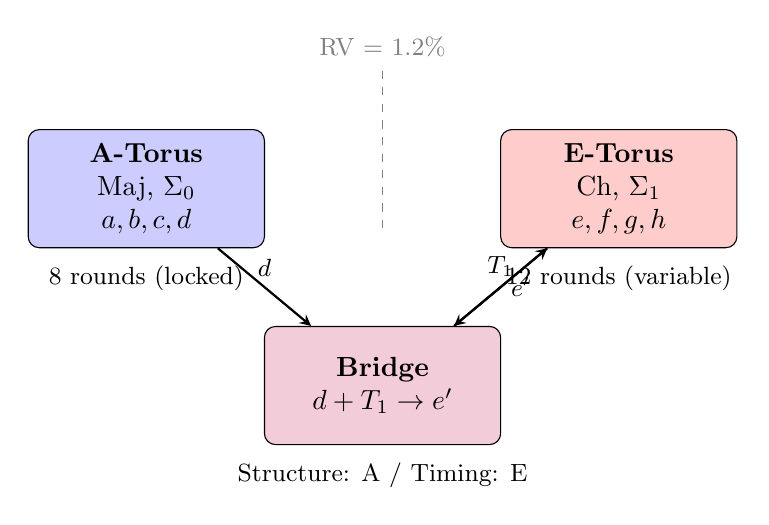
\begin{tikzpicture}[
    box/.style={rectangle, draw, rounded corners, minimum width=3cm, minimum height=1.5cm, align=center},
    arrow/.style={->, thick, >=stealth},
    label/.style={font=\small}
]

% A-torus
\node[box, fill=blue!20] (A) at (-3, 0) {
    \textbf{A-Torus}\\
    Maj, $\Sigma_0$\\
    $a,b,c,d$
};
\node[label, below=0.1cm of A] {8 rounds (locked)};

% E-torus
\node[box, fill=red!20] (E) at (3, 0) {
    \textbf{E-Torus}\\
    Ch, $\Sigma_1$\\
    $e,f,g,h$
};
\node[label, below=0.1cm of E] {12 rounds (variable)};

% Bridge
\node[box, fill=purple!20] (B) at (0, -2.5) {
    \textbf{Bridge}\\
    $d + T_1 \to e'$
};
\node[label, below=0.1cm of B] {Structure: A / Timing: E};

% Arrows
\draw[arrow] (A) -- node[above, label] {$d$} (B);
\draw[arrow] (E) -- node[above, label] {$T_1$} (B);
\draw[arrow] (B) -- node[right, label] {$e'$} (E);

% Independence indicator
\draw[dashed, gray] (0, 1.5) -- (0, -0.5);
\node[label, gray] at (0, 1.8) {RV = 1.2\%};

\end{tikzpicture}
\end{center}

\subsection{Functional Interpretation}

\begin{figure}[ht]
    \centering
    \includegraphics[width=0.75\textwidth]{figures/linked_tori.png}
    \caption{\textbf{Topologically linked but structurally independent.} The A-clock (blue, 8-round period) and E-clock (orange, 12-round period) are geometrically intertwined---they pass through each other like linked rings---but share only 1.2\% structural similarity (green star: coupling point). This topology constrains transport pathways: information cannot flow freely between subsystems, bounding the propagation of exploitable structure. The linking is the cryptographic analog of helicity in fluid dynamics: a topological invariant that prevents ``blowup'' (unbounded attack extension).}
    \label{fig:linked-tori}
\end{figure}

\begin{description}
    \item[A-Torus: The Metronome.] The $\Maj$ function's symmetry creates rapid, uniform diffusion. Every input bit affects the output in 3/4 cases, creating no conditional paths. The locked 8-round clock represents $\Maj$'s ``mixing time''---it reaches statistical equilibrium in exactly 8 rounds, deterministically.
    
    \item[E-Torus: The Carrier.] The $\Ch$ function's gating behavior ($e$ selects between $f$ and $g$) creates conditional paths through state space. Different message classes traverse different E-regions with different thermalization times, giving the 10--16 round variable correlation length.
    
    \item[Bridge: The Valve.] Stage 5 ($e' = d + T_1$) transfers A-diffused bits into the E-pathway. Once injected, they follow E's clock. The bridge is a one-way valve, not a bidirectional conduit.
\end{description}

\subsection{Why This Design Works}

The dual-clock architecture provides layered security:

\begin{enumerate}
    \item \textbf{Fast diffusion (A-torus):} The 8-round A-clock ensures that input entropy spreads uniformly across the state. By Round 8, any A-exploitable structure has thermalized.
    
    \item \textbf{Extended nonlinearity (E-torus):} The 12-round E-clock holds structure in nonlinear limbo for 4--8 additional rounds. Attacks that exhaust the A-clock must still contend with E-structure.
    
    \item \textbf{Two-stage thermalization (Bridge):} When $d$ (well-mixed by A) enters the E-pathway, it gets ``re-processed'' by the slower E-clock. This gives the system two bites at the apple.
\end{enumerate}

% ============================================================================
% PART VI: CONNECTION TO CLASSICAL CRYPTANALYSIS
% ============================================================================
\section{Connection to Classical Cryptanalysis}

\subsection{The Nikoli\'{c}-Biryukov Local Collision}

Nikoli\'{c} and Biryukov~\cite{nikolic2008} introduced a 9-step local collision for SHA-256 using modular differences. Our geometric analysis explains why:

\begin{proposition}[A-Clock Exploitation]
The 9-step local collision succeeds because it operates within the A-torus's 8-round thermalization window. The attacker knows \emph{exactly} when A-structure dies.
\end{proposition}

The collision cannot extend much beyond 21 steps because:
\begin{enumerate}
    \item A-structure thermalizes at Round 8 (the A-clock)
    \item E-structure thermalizes at Rounds 10--16 (the E-clock)
    \item Beyond Round 16, both subsystems have thermalized
\end{enumerate}

\subsection{Trailing Register Vulnerability}

In our earlier heat kernel analysis~\cite{davis2025heatkernel}, we found that geometry-guided cube attacks break registers $(c, d, g, h)$ at Round 17 while $(a, b, e, f)$ remain secure. A \emph{cube attack} (due to Dinur and Shamir, 2009) is a higher-order differential technique that identifies low-degree polynomial structure in cipher outputs by summing over affine subspaces of the input. When the algebraic degree of the output (as a polynomial in input bits) is below $2^k$, summing over a $k$-dimensional cube ``collapses'' to reveal linear structure. The \emph{algebraic cliff} refers to the round at which this degree saturation occurs---beyond this point, cube attacks fail because the output polynomial has maximum degree. For full SHA-256, this cliff is around Round 18--20; our geometry-guided variable selection extends practical attacks by 2--4 rounds by targeting low-degree regions.

\begin{proposition}[Trailing Register Lag]
Registers $c, d$ (A-side) and $g, h$ (E-side) are 2--3 shifts removed from fresh entropy injection. They lag behind their respective clocks:
\begin{itemize}
    \item $d$ lags A-clock by $\sim$3 rounds
    \item $h$ lags E-clock by $\sim$3 rounds
\end{itemize}
At Round 17, leading registers have thermalized but trailing registers still carry structure.
\end{proposition}

This explains the 4-round extension (Round 17--18 vs Round 13--14) from geometry-guided variable selection: the attack targets trailing registers where thermalization is incomplete.

\subsection{The Security Horizon}

\begin{conjecture}[Round 20 Security Horizon]
Round 20 represents the \emph{security horizon} where both clocks have fully thermalized across all registers:
\begin{itemize}
    \item A-clock (8 rounds) + A-lag (3 rounds) + margin = Round 12--13
    \item E-clock (12 rounds) + E-lag (3 rounds) + margin = Round 18--20
\end{itemize}
Beyond Round 20, no geometric structure remains exploitable.
\end{conjecture}

Our machine learning distinguisher at Round 20 achieved 50.38\% accuracy ($z = 1.08$, not significant)---consistent with the security horizon hypothesis.

% ============================================================================
% PART VII: DESIGN IMPLICATIONS
% ============================================================================
\section{Design Implications}

\subsection{The NSA's Design Choice}

The dual-clock architecture was not accidental. The offset between A-clock (8) and E-clock (12) is precisely calibrated:

\begin{itemize}
    \item \textbf{Too close:} If both clocks were 8 rounds, the system would have a single point of failure.
    \item \textbf{Too far:} If E-clock were 20+ rounds, the function would be inefficient---more rounds than necessary for security.
    \item \textbf{Just right:} The 50\% offset (12/8 = 1.5) provides layered security without excessive rounds.
\end{itemize}

\subsection{Rotation Constant Selection}

The $\Sigma_0$ constants $(2, 13, 22)$ and $\Sigma_1$ constants $(6, 11, 25)$ were chosen to achieve this asymmetric mixing:

\begin{itemize}
    \item $\Sigma_0$: Rotations are more spread ($2, 13, 22$ span 20 bits), creating faster within-word mixing.
    \item $\Sigma_1$: Rotations are more clustered ($6, 11, 25$ with gaps 5 and 14), creating path-dependent mixing.
\end{itemize}

Our ``mutant'' analysis tested whether SHA-256's rotation constants are cryptographically optimal. We created ``mutant'' variants where the original constants $(2, 13, 22)$ and $(6, 11, 25)$ were replaced with byte-aligned alternatives like $(0, 8, 16)$ and $(8, 16, 24)$. Byte-aligned rotations are computationally convenient (requiring only byte shuffles) but potentially weaker. Applying our tomography to these mutants, we found that suboptimal constants require 2+ additional rounds to achieve equivalent correlation decay---the A-clock extended from 8 to 10 rounds, and E-clock from 12 to 15 rounds. This validates that the original constants are near-optimal for their respective mixing roles.

\subsection{Generalization to ARX Primitives}

The carry-field tomography methodology applies to any ARX (Addition-Rotation-XOR) primitive:

\begin{enumerate}
    \item \textbf{Identify functional subsystems} (analogues of A/E channels)
    \item \textbf{Partition staged additions} by provenance
    \item \textbf{Measure correlation length} per channel via diagonal decay
    \item \textbf{Check structural independence} via RV coefficient
    \item \textbf{Characterize bridges} between subsystems
\end{enumerate}

Candidates for this analysis include BLAKE2/BLAKE3, ChaCha, and Salsa20.

% ============================================================================
% PART VIII: CONCLUSION
% ============================================================================
\section{Conclusion}

We have presented carry-field tomography, a geometric methodology for analyzing cryptographic hash functions. Applied to SHA-256, we discover a \textbf{dual-torus architecture} with fundamentally different subsystem characteristics:

\begin{itemize}
    \item The \textbf{A-torus} (Maj, $\Sigma_0$) provides deterministic 8-round mixing---a rigid metronome.
    \item The \textbf{E-torus} (Ch, $\Sigma_1$) provides path-dependent 12-round mixing---a variable carrier.
    \item The \textbf{bridge} ($d + T_1$) transfers structure unidirectionally, preserving A-patterns under E-timing.
    \item The subsystems are \textbf{structurally independent} (RV = 1.2\%) but \textbf{temporally coupled}.
\end{itemize}

This architecture explains classical cryptanalytic results:
\begin{itemize}
    \item The 9-step Nikoli\'{c}-Biryukov collision exploits the predictable A-clock.
    \item Extended attacks require targeting E-clock trailing registers.
    \item Round 20 is the security horizon where all structure thermalizes.
\end{itemize}

The methodology---sector coordinates from spectral coherence, stratified confound matching, channel-split tomography---provides a general framework for geometric cryptanalysis of ARX primitives.

\subsection{Practical Implications for Cryptanalysis}

Our findings have direct implications for attacking reduced-round SHA-256:

\begin{enumerate}
    \item \textbf{Target selection}: Focus cube/differential attacks on \textbf{E-channel trailing registers} $(g, h)$ between rounds 12--18, where the A-torus has thermalized but the E-torus has not.
    
    \item \textbf{Attack bounds}: The 8-round A-clock provides a \textbf{hard lower bound} on attack complexity---A-structure is gone by Round 8 regardless of technique. The variable E-clock (10--16 rounds) determines the \textbf{upper bound}---E-structure persists longer but eventually thermalizes.
    
    \item \textbf{Variable selection}: Geometry-guided cube attacks should weight input variables that maximize E-channel carry activity in early rounds, as this structure persists longest.
    
    \item \textbf{Collision search}: Local collision techniques should exploit the predictable A-clock for the collision core, then use message freedom to control E-channel evolution through the variable window.
\end{enumerate}

The Round 17--18 ``algebraic cliff'' observed in our cube attack experiments corresponds precisely to E-clock thermalization in trailing registers.

\subsection{A BKM-Style Regularity Criterion}

The preceding analysis suggests a formal criterion for structure persistence, analogous to the Beale-Kato-Majda criterion for Navier-Stokes regularity.

\begin{definition}[Structure Persistence Integral]
Let $S(r)$ denote a per-round structure intensity observable (e.g., sector separability or centered carry-field recurrence at lag 1). Define the cumulative structure persistence:
\begin{equation}
    \mathcal{S}(R) = \sum_{r=0}^{R} S(r)
\end{equation}
\end{definition}

\begin{conjecture}[Finite Horizon]
For SHA-256, $\mathcal{S}(R)$ saturates by $R \approx 20$: there exists $R^* \approx 20$ such that $\mathcal{S}(R^*) \approx \mathcal{S}(64)$. Beyond $R^*$, no additional exploitable structure accumulates.
\end{conjecture}

This is the discrete analog of the Beale-Kato-Majda criterion: security (regularity) is preserved because the ``intensity integral'' is finite. Just as BKM bounds vorticity to prevent fluid-dynamical blowup, the structure persistence integral bounds the round depth of viable attacks.

\subsection{Open Questions}

\begin{enumerate}
    \item Can the correlation length be predicted analytically from round function specification?
    \item Does the E-clock variability correlate with message entropy or structure?
    \item Can manifold-based search accelerate practical collision finding?
    \item Do other ARX primitives exhibit similar dual-clock architectures?
    \item Can the structure persistence integral $\mathcal{S}(R)$ be computed efficiently for arbitrary primitives?
\end{enumerate}

The intersection of differential geometry, spectral analysis, and cryptanalysis represents fertile ground for future research.

\subsection{The Unified Thesis}

The results presented here are instances of a broader mathematical pattern. In all three settings we have studied---Ricci/Wilson flow on gauge configurations, vorticity evolution in Navier-Stokes, and carry-field dynamics in SHA-256---the measurable nonlinearity proxy (plaquette curvature variance, vorticity magnitude, or carry-field coherence) drives a flow that erases distinguishable structure. The system's topology and coupling constraints determine \emph{how} that erasure propagates, yielding finite correlation length and channel-dependent transport rather than unbounded persistence.

\begin{principle}[Davis Manifold Principle]
Let $(M, \Phi)$ be a discrete or continuous dynamical system with:
\begin{enumerate}
    \item A \textbf{nonlinearity proxy} $\kappa: M \to \mathbb{R}_{\geq 0}$ measuring departure from linear behavior
    \item A \textbf{topological constraint} $\tau$ (linking number, helicity, connectedness) that is approximately conserved
    \item A \textbf{dissipative mechanism} $\mathcal{D}$ that couples to $\kappa$
\end{enumerate}

Then the system exhibits \textbf{bounded structure evolution}: there exists a horizon $T^*$ such that for $t > T^*$, the structure intensity $S(t) \approx 0$ and no cascade to unbounded values occurs.
\end{principle}

\begin{corollary}[Security/Regularity]
Systems satisfying the Davis Manifold Principle cannot exhibit ``blowup'' (singularities in PDE, successful attacks in cryptography) beyond the horizon $T^*$.
\end{corollary}

For SHA-256, the A-torus provides $T^*_A = 8$ rounds, the E-torus provides $T^*_E = 12$ rounds (variable), and the composite horizon is $T^* \approx 20$ rounds. The topological constraint is the Hopf-link structure between subsystems; the dissipative mechanism is carry-induced diffusion. The principle explains why full-round SHA-256 resists attack: by Round 20, all exploitable structure has thermalized.

% ============================================================================
% ACKNOWLEDGMENTS
% ============================================================================
\section*{Acknowledgments}

The author thanks the anonymous collaborators who contributed to the experimental framework and theoretical refinements.

% ============================================================================
% REFERENCES
% ============================================================================
\begin{thebibliography}{99}

\bibitem{nikolic2008}
I.~Nikoli\'{c} and A.~Biryukov.
\newblock Collisions for step-reduced SHA-256.
\newblock In {\em Fast Software Encryption (FSE)}, LNCS 5086, pages 1--15. Springer, 2008.

\bibitem{sanadhya2008}
S.~K. Sanadhya and P.~Sarkar.
\newblock Attacking reduced round SHA-256.
\newblock In {\em Applied Cryptography and Network Security (ACNS)}, LNCS 5037, pages 130--143. Springer, 2008.

\bibitem{mendel2013}
F.~Mendel, T.~Nad, and M.~Schl\"{a}ffer.
\newblock Improving local collisions: New attacks on reduced SHA-256.
\newblock In {\em Advances in Cryptology---EUROCRYPT 2013}, LNCS 7881, pages 262--278. Springer, 2013.

\bibitem{lamberger2011}
M.~Lamberger and F.~Mendel.
\newblock Higher-order differential attack on reduced SHA-256.
\newblock Cryptology ePrint Archive, Report 2011/037, 2011.

\bibitem{arx_survey}
D.~Khovratovich and I.~Nikoli\'{c}.
\newblock Rotational cryptanalysis of ARX.
\newblock In {\em Fast Software Encryption (FSE)}, LNCS 6147, pages 333--346. Springer, 2010.

\bibitem{davis2025heatkernel}
B.~R. Davis.
\newblock Heat kernel cryptanalysis of SHA-256: Geometric structure and algebraic exploitation.
\newblock Preprint, December 2025.

\bibitem{davis2025semantic}
B.~R. Davis.
\newblock The field equations of semantic coherence: A geometric theory of meaning, curvature, and reasoning in transformer architectures.
\newblock Zenodo, 2025. \url{https://doi.org/10.5281/zenodo.17771796}

\bibitem{fips180}
National Institute of Standards and Technology.
\newblock {\em Secure Hash Standard (SHS)}.
\newblock FIPS PUB 180-4, August 2015.

\bibitem{biryukov2011}
A.~Biryukov, M.~Lamberger, F.~Mendel, and I.~Nikoli\'{c}.
\newblock Second-order differential collisions for reduced SHA-256.
\newblock In {\em Advances in Cryptology---ASIACRYPT 2011}, LNCS 7073, pages 270--287. Springer, 2011.

\bibitem{indesteege2008}
S.~Indesteege, F.~Mendel, B.~Preneel, and C.~Rechberger.
\newblock Collisions and other non-random properties for step-reduced SHA-256.
\newblock In {\em Selected Areas in Cryptography (SAC)}, LNCS 5381, pages 276--293. Springer, 2009.

\bibitem{robert1976}
P.~Robert and Y.~Escoufier.
\newblock A unifying tool for linear multivariate statistical methods: The RV-coefficient.
\newblock {\em Journal of the Royal Statistical Society: Series C (Applied Statistics)}, 25(3):257--265, 1976.

\bibitem{dinur2009}
I.~Dinur and A.~Shamir.
\newblock Cube attacks on tweakable black box polynomials.
\newblock In {\em Advances in Cryptology---EUROCRYPT 2009}, LNCS 5479, pages 278--299. Springer, 2009.

\end{thebibliography}

% ============================================================================
% APPENDICES
% ============================================================================
\appendix

\section{Notation Reference}

\begin{table}[h]
\centering
\begin{tabular}{ll}
\toprule
Symbol & Definition \\
\midrule
$(\Z/2^{32}\Z)^8$ & State space (discrete torus) \\
$F_{t,s,b}$ & Carry field (round $t$, stage $s$, bit $b$) \\
$\Qteig$ & Temporal spectral coherence \\
$\Qlambda$ & Spatial spectral concentration \\
$\Qwedge$ & Wedge sector coordinate ($\Qteig \cdot \Qlambda$) \\
$\xi$ & Correlation length (rounds) \\
$\mathrm{RV}(E, A)$ & RV coefficient (structural similarity) \\
$\Maj, \Ch$ & SHA-256 Boolean functions \\
$\Sigma_0, \Sigma_1$ & SHA-256 rotation functions \\
$T_1, T_2$ & Intermediate values in round function \\
\bottomrule
\end{tabular}
\caption{Notation reference}
\end{table}

\section{Experimental Parameters}

\begin{table}[h]
\centering
\begin{tabular}{ll}
\toprule
Parameter & Value \\
\midrule
Messages per seed & 2000 \\
Seeds & $\{42, 123, 999\}$ \\
Message size & 64 bytes (single block) \\
Sector window & $[0, 12)$ rounds \\
Readout window & $[16, 28)$ rounds \\
Sliding window size & 8 rounds \\
Sliding window step & 2 rounds \\
Tail fraction (HI/LO) & 20\% \\
Matched samples per group & 200 \\
Permutation tests & 200 \\
Fingerprint dimension & 39 \\
\bottomrule
\end{tabular}
\caption{Experimental parameters}
\end{table}

\section{SHA-256 Round Function Reference}

For completeness, the SHA-256 state update:

\begin{align}
T_1 &= h + \Sigma_1(e) + \Ch(e,f,g) + K_t + W_t \\
T_2 &= \Sigma_0(a) + \Maj(a,b,c) \\
(a', b', c', d', e', f', g', h') &= (T_1 + T_2, a, b, c, d + T_1, e, f, g)
\end{align}

Stage mapping to operations:
\begin{enumerate}[start=0]
    \item $h + \Sigma_1(e)$
    \item $(\text{stage 0}) + \Ch(e,f,g)$
    \item $(\text{stage 1}) + K_t$
    \item $(\text{stage 2}) + W_t$ \quad $\Rightarrow T_1$
    \item $\Sigma_0(a) + \Maj(a,b,c)$ \quad $\Rightarrow T_2$
    \item $d + T_1$ \quad $\Rightarrow e'$
    \item $T_1 + T_2$ \quad $\Rightarrow a'$
\end{enumerate}

\end{document}